
%(BEGIN_QUESTION)
% Copyright 2006, Tony R. Kuphaldt, released under the Creative Commons Attribution License (v 1.0)
% This means you may do almost anything with this work of mine, so long as you give me proper credit

A {\it strain gauge} is an array constructed from thin metal film designed to increase resistance as it is stretched and decrease resistance as it is compressed.  Strain gauges are typically bonded to metal specimens undergoing mechanical testing, as a means of sensing how much strain is being applied to that metal specimen.  In order to translate the resistance of the strain gauge into a measurable voltage signal, the strain gauge is typically incorporated into one arm of a ``bridge'' circuit.

\vskip 10pt

The following bridge circuit uses two strain gauges (one to measure strain, the other to compensate for temperature changes), the amount of strain indicated by the voltmeter in the center of the bridge.  Unfortunately, though, it has a problem.  Instead of registering a very small voltage as it normally does, the voltmeter is ``pegged'' (driven beyond its normal full-range measurement) by a large voltage difference, with point {\bf B} positive and point {\bf A} negative as shown here:

$$\includegraphics[width=15.5cm]{i00188x01.eps}$$

\goodbreak
Something is wrong in the bridge circuit, because this voltage is present even when there is no physical stress on the specimen.  Identify which of the following faults could cause the excessive voltage to appear across the voltmeter, and which could not.  Consider only one of these faults at a time (no multiple, simultaneous faults):

% No blank lines allowed between lines of an \halign structure!
% I use comments (%) instead, so that TeX doesn't choke.

$$\vbox{\offinterlineskip
\halign{\strut
\vrule \quad\hfil # \ \hfil & 
\vrule \quad\hfil # \ \hfil & 
\vrule \quad\hfil # \ \hfil \vrule \cr
\noalign{\hrule}
%
% First row
{\bf Fault} & {\bf Possible} & {\bf Impossible} \cr
%
\noalign{\hrule}
%
% Another row
$R_1$ failed open &  &  \cr
%
\noalign{\hrule}
%
% Another row
$R_2$ failed open &  &  \cr
%
\noalign{\hrule}
%
% Another row
Strain gauge failed open &  &  \cr
%
\noalign{\hrule}
%
% Another row
Dummy gauge failed open &  &  \cr
%
\noalign{\hrule}
%
% Another row
$R_1$ failed shorted &  &  \cr
%
\noalign{\hrule}
%
% Another row
$R_2$ failed shorted &  &  \cr
%
\noalign{\hrule}
%
% Another row
Strain gauge failed shorted &  &  \cr
%
\noalign{\hrule}
%
% Another row
Dummy gauge failed shorted &  &  \cr
%
\noalign{\hrule}
%
% Another row
Voltage source dead &  &  \cr
%
\noalign{\hrule}
} % End of \halign 
}$$ % End of \vbox

\vskip 20pt \vbox{\hrule \hbox{\strut \vrule{} {\bf Suggestions for Socratic discussion} \vrule} \hrule}

\begin{itemize}
\item{} Identify which fundamental principles of electric circuits apply to each step of your analysis of this circuit.  In other words, be prepared to explain the reason(s) ``why'' for every step of your analysis, rather than merely describing those steps.
\item{} Explain why the two strain gauge elements are orthogonally bonded (i.e. attached 90$^{o}$ to each other) to the specimen.
\end{itemize}

\underbar{file i00188}
%(END_QUESTION)





%(BEGIN_ANSWER)

\noindent
{\bf Partial answer:}

% No blank lines allowed between lines of an \halign structure!
% I use comments (%) instead, so that TeX doesn't choke.

$$\vbox{\offinterlineskip
\halign{\strut
\vrule \quad\hfil # \ \hfil & 
\vrule \quad\hfil # \ \hfil & 
\vrule \quad\hfil # \ \hfil \vrule \cr
\noalign{\hrule}
%
% First row
{\bf Fault} & {\bf Possible} & {\bf Impossible} \cr
%
\noalign{\hrule}
%
% Another row
$R_1$ failed open & $\surd$ &  \cr
%
\noalign{\hrule}
%
% Another row
$R_2$ failed open &  &  \cr
%
\noalign{\hrule}
%
% Another row
Strain gauge failed open &  & $\surd$ \cr
%
\noalign{\hrule}
%
% Another row
Dummy gauge failed open &  &  \cr
%
\noalign{\hrule}
%
% Another row
$R_1$ failed shorted &  &  \cr
%
\noalign{\hrule}
%
% Another row
$R_2$ failed shorted &  &  \cr
%
\noalign{\hrule}
%
% Another row
Strain gauge failed shorted &  &  \cr
%
\noalign{\hrule}
%
% Another row
Dummy gauge failed shorted &  &  \cr
%
\noalign{\hrule}
%
% Another row
Voltage source dead &  & $\surd$ \cr
%
\noalign{\hrule}
} % End of \halign 
}$$ % End of \vbox

%(END_ANSWER)





%(BEGIN_NOTES)

% No blank lines allowed between lines of an \halign structure!
% I use comments (%) instead, so that TeX doesn't choke.

$$\vbox{\offinterlineskip
\halign{\strut
\vrule \quad\hfil # \ \hfil & 
\vrule \quad\hfil # \ \hfil & 
\vrule \quad\hfil # \ \hfil \vrule \cr
\noalign{\hrule}
%
% First row
{\bf Fault} & {\bf Possible} & {\bf Impossible} \cr
%
\noalign{\hrule}
%
% Another row
$R_1$ failed open & $\surd$ &  \cr
%
\noalign{\hrule}
%
% Another row
$R_2$ failed open &  & $\surd$ \cr
%
\noalign{\hrule}
%
% Another row
Strain gauge failed open &  & $\surd$ \cr
%
\noalign{\hrule}
%
% Another row
Dummy gauge failed open & $\surd$ &  \cr
%
\noalign{\hrule}
%
% Another row
$R_1$ failed shorted &  & $\surd$ \cr
%
\noalign{\hrule}
%
% Another row
$R_2$ failed shorted & $\surd$ &  \cr
%
\noalign{\hrule}
%
% Another row
Strain gauge failed shorted & $\surd$ &  \cr
%
\noalign{\hrule}
%
% Another row
Dummy gauge failed shorted &  & $\surd$ \cr
%
\noalign{\hrule}
%
% Another row
Voltage source dead &  & $\surd$ \cr
%
\noalign{\hrule}
} % End of \halign 
}$$ % End of \vbox

This question helps students build the skill of eliminating unlikely fault possibilities, allowing them to concentrate instead on what is more likely.  An important skill in system troubleshooting is the ability to formulate probabilities for various fault scenarios.  Without this skill, you will waste a lot of time looking for unlikely faults, thereby wasting time.

For each fault scenario it is important to ask your students {\it why} they think it is possible or not possible.  It might be that some students get the right answer(s) for the wrong reasons, so it is good to explore the reasoning for each answer.

\filbreak

$$\includegraphics[width=15.5cm]{i00188x02.eps}$$

\vskip 20pt \vbox{\hrule \hbox{\strut \vrule{} {\bf Virtual Troubleshooting} \vrule} \hrule}

This question is a good candidate for a ``Virtual Troubleshooting'' exercise.  Presenting the diagram to students, you first imagine in your own mind a particular fault in the system.  Then, you present one or more symptoms of that fault (something noticeable by an operator or other user of the system).  Students then propose various diagnostic tests to perform on this system to identify the nature and location of the fault, as though they were technicians trying to troubleshoot the problem.  Your job is to tell them what the result(s) would be for each of the proposed diagnostic tests, documenting those results where all the students can see.

During and after the exercise, it is good to ask students follow-up questions such as:

\begin{itemize}
\item{} What does the result of the last diagnostic test tell you about the fault?
\item{} Suppose the results of the last diagnostic test were different.  What then would that result tell you about the fault?
\item{} Is the last diagnostic test the best one we could do?
\item{} What would be the ideal order of tests, to diagnose the problem in as few steps as possible?
\end{itemize}

%INDEX% Measurement, strain gauge

%(END_NOTES)


